\begin{flushright}
    در این جلسه به بررسی بهینه‌سازی در فضای پیوسته میپردازیم.
    در ابتدا یک مثال از بهینه‌سازی پیوسته را میبینیم.
    فرض کنید میخواهیم مکان یک فرودگاه را طوری پیدا کنیم که فاصله آن از چندین شهر کمینه باشد.
    در نتیجه فرم بهینه‌سازی ما به شکل زیر در می آید:

    \begin{displaymath}
        \centering
        minimize\ \sum_{i=1}^{m}\left|\left|x-y^{\left(m\right)}\right|\right|
    \end{displaymath}

    دلیل استفاده از بهینه‌سازی:
    خیلی اوقات مسائل ما در نهایت به فرم یک مسئله بهینه‌سازی در می آید.
    به همین دلیل میتوانیم روند حل مسئله و تعریف آن را و حل مسئله بهینه‌سازی را دو مسئله جدا بکنیم.
    به همین دلیل ما دوست داریم مسائل را به یک سری فرم های معروف بهینه‌سازی ماننده LinearProgramming، QuadraticProgramming و \ldots برسیم.
    مسائل optimization را میتوان به 4 دسته تقسیم کرد.
    \begin{enumerate}
        \item براساس محدب بودن: ممکن است مسئله بهینه‌سازی ما محدب یا غیر محدب باشد.
        \item براساس قیود: ممکن است مسئله بهینه‌سازی ما مقید یا بدون قید باشد.
    \end{enumerate}

    \begin{figure}[H]
        \centering
        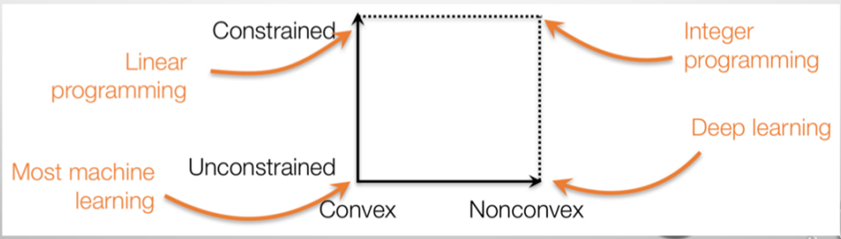
\includegraphics[width=0.8\textwidth]{source/opt-types.png}
        \label{fig:optimization}
    \end{figure}

    به طور کلی مسائل بهینه‌سازی راه حل کلی ندارند و غیرقابل حل هستند.
    برای قابل حل کردن و به دست آوردن فرم های کلی تر ما مسائل بهینه‌سازی را محدود میکنیم و روی نوع تابع بهینه‌سازی قید میگذاریم.
    یکی از این قیود پیوستگی لیبشیتز (Lipschitz-continuous) است.
    پیوستگی لیبشیتز به این معنی است که خط مماس بر تابع وشیب تابع همواره بین 2 خط با شیب L و -L قرار بگیرد.
    درواقع به صورت فرم ریاضی میتوان گفت یک L وجود داشته باشد به طوریکه :

    \begin{displaymath}
        \left|f\left(x\right)-f\left(y\right)\right|\le L\ |\left|x-y\right||
    \end{displaymath}

    برای مثال تابع $e^x$ دارای این شرط نیست.
    به طوری کلی اگر بتوانیم حد بالایی برای مشتق تابع پیدا کنیم L همان حد بالای مشتق است.
    می توان نشان داد برای توابع لیبشیتز پیوسته بعد از t مرحله خطای ما از اردر $\Omega(\frac{1}{t^\frac{1}{n}})$  است.

    \subsubject{convex}{files/convex.tex}
    \subsubject{descent gradient}{files/gradient.tex}
\end{flushright}
